\chapter{Clase 1: Variables bidimensionales y distribuciones de frecuencias}

\section{Variables estadísticas multidimensionales}

En un estudio, cada individuo, objeto o unidad observada puede describirse mediante una o varias características. Una \textbf{variable estadística $k$-dimensional} reúne $k$ variables medidas sobre las mismas unidades y se representa por

\begin{equation*}
\vec{X}=(X_1,X_2,\ldots,X_k).
\end{equation*}

Para la unidad $r$, la observación correspondiente es el vector

\begin{equation*}
\vec{x}_r=(x_{r1},x_{r2},\ldots,x_{rk}),\qquad r=1,2,\ldots,n,
\end{equation*}

que contiene los valores registrados de las $k$ variables para esa unidad. El número $k$ indica cuántas características se estudian conjuntamente; $n$ es el número de unidades observadas.

\begin{figure}[H]
\centering
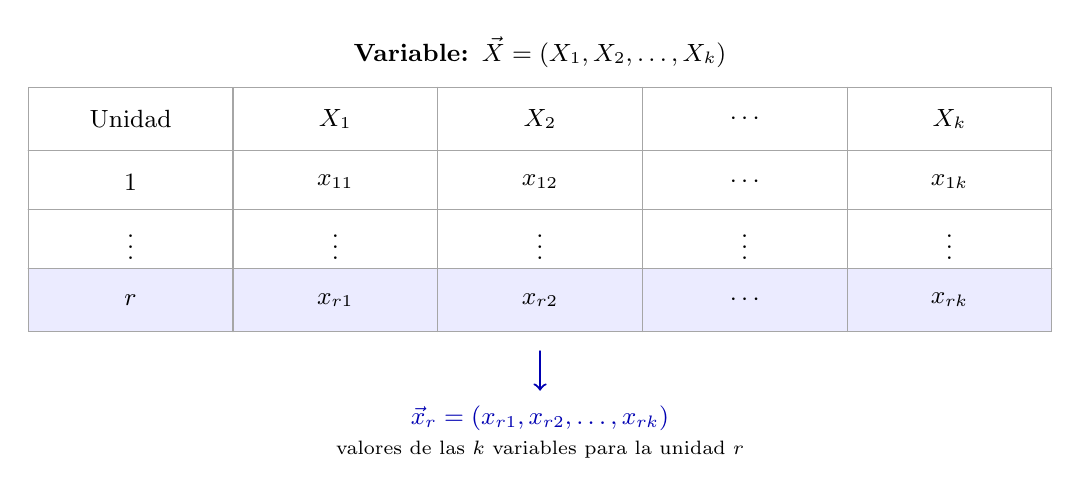
\begin{tikzpicture}[every node/.style={font=\small}, line cap=round]
    % Cada fila representa una unidad y cada columna una variable.
    \node[font=\small\bfseries] at (0,2.35)
        {Variable: $\vec{X}=(X_1,X_2,\ldots,X_k)$};

    % La fila r se destaca para mostrar sus k mediciones.
    \path[fill=blue!8] (-6.5,-1.2) rectangle (6.5,-0.4);
    \draw[gray!70] (-6.5,-1.2) rectangle (6.5,1.9);
    \foreach \x in {-3.9,-1.3,1.3,3.9}
        \draw[gray!70] (\x,-1.2) -- (\x,1.9);
    \foreach \y in {1.1,0.35,-0.4}
        \draw[gray!70] (-6.5,\y) -- (6.5,\y);

    \node at (-5.2,1.5) {Unidad};
    \node at (-2.6,1.5) {$X_1$};
    \node at (0,1.5) {$X_2$};
    \node at (2.6,1.5) {$\cdots$};
    \node at (5.2,1.5) {$X_k$};

    \node at (-5.2,0.7) {$1$};
    \node at (-2.6,0.7) {$x_{11}$};
    \node at (0,0.7) {$x_{12}$};
    \node at (2.6,0.7) {$\cdots$};
    \node at (5.2,0.7) {$x_{1k}$};

    \node at (-5.2,-0.025) {$\vdots$};
    \node at (-2.6,-0.025) {$\vdots$};
    \node at (0,-0.025) {$\vdots$};
    \node at (2.6,-0.025) {$\vdots$};
    \node at (5.2,-0.025) {$\vdots$};

    \node[font=\small\bfseries] at (-5.2,-0.8) {$r$};
    \node[font=\small\bfseries] at (-2.6,-0.8) {$x_{r1}$};
    \node[font=\small\bfseries] at (0,-0.8) {$x_{r2}$};
    \node[font=\small\bfseries] at (2.6,-0.8) {$\cdots$};
    \node[font=\small\bfseries] at (5.2,-0.8) {$x_{rk}$};

    \draw[->,thick,blue!70!black] (0,-1.45) -- (0,-1.95);
    \node[font=\small\bfseries,text=blue!70!black] at (0,-2.3)
        {$\vec{x}_r=(x_{r1},x_{r2},\ldots,x_{rk})$};
    \node[font=\scriptsize] at (0,-2.7) {valores de las $k$ variables para la unidad $r$};
\end{tikzpicture}
\caption{La fila de la unidad $r$ reúne los valores observados de las $k$ variables y forma el vector $\vec{x}_r$.}
\label{fig:variable-k-dimensional}
\end{figure}

\subsection{Variable estadística bidimensional}

Cuando se estudian dos características en cada unidad, se tiene una \textbf{variable estadística bidimensional}. La representaremos mediante

$$
(X,Y).
$$

En una muestra de $n$ unidades, los datos son los pares

$$
(x_1,y_1),(x_2,y_2),\ldots,(x_n,y_n),
$$

donde $x_r$ y $y_r$ corresponden siempre a la misma unidad $r$. En esta clase nos centraremos en describir cómo se distribuyen conjuntamente dos variables, sin perder la correspondencia entre sus observaciones.

\subsection{Tipos de variables y ejemplos}

Cada componente de $(X,Y)$ puede ser cuantitativa o cualitativa. Las variables cuantitativas expresan conteos o mediciones; las cualitativas identifican categorías. La siguiente tabla resume ejemplos:

\begin{table}[H]
\centering
\small
\renewcommand{\arraystretch}{1.15}
\begin{tabular}{|>{\raggedright\arraybackslash}p{4cm}|>{\raggedright\arraybackslash}p{4.1cm}|>{\raggedright\arraybackslash}p{6.3cm}|}
\hline
\textbf{Tipo de variable} & \textbf{Ejemplo} & \textbf{Valores posibles} \\ \hline
Cuantitativa discreta & Número de visitas al cine en un mes & $0,1,2,3,\ldots$ \\ \hline
Cuantitativa continua & Tiempo de traslado al trabajo & Cualquier valor no negativo, por ejemplo $18.5$ minutos \\ \hline
Cualitativa nominal & Color de ojos & Café, miel, verde, azul \\ \hline
Cualitativa ordinal & Nivel de satisfacción & Bajo, medio, alto \\ \hline
\end{tabular}
\caption{Ejemplos de tipos de variables estadísticas.}
\label{tab:tipos-variables}
\end{table}

La clasificación depende de lo que representa cada variable, no de la forma en que se escriben sus valores. Por ejemplo, asignar números a categorías no convierte una variable cualitativa en cuantitativa.

\section{Distribuciones de frecuencias conjuntas}

Una \textbf{distribución de frecuencias} organiza y resume los datos indicando cuántas observaciones corresponden a cada valor o categoría. Para dos variables, la \textbf{distribución de frecuencias conjunta} presenta las frecuencias de cada combinación de valores de $X$ y de $Y$.

Sean

$$
(x_1,y_1),(x_2,y_2),\ldots,(x_n,y_n)
$$

Las observaciones anteriores conforman la muestra. Supongamos que las modalidades o clases de $X$ y de $Y$ son, respectivamente:

$$
X:\quad c_1,c_2,\ldots,c_m,\qquad Y:\quad d_1,d_2,\ldots,d_k.
$$

La celda $(i,j)$ de la tabla corresponde a la combinación $(c_i,d_j)$.

\subsection{Frecuencia absoluta conjunta}

La \textbf{frecuencia absoluta conjunta} $n_{ij}$ cuenta cuántas unidades presentan simultáneamente la modalidad $c_i$ de $X$ y la modalidad $d_j$ de $Y$:

$$
n_{ij}=\#\{r: x_r=c_i\text{ e }y_r=d_j\}.
$$

Si los datos están agrupados, $x_r=c_i$ e $y_r=d_j$ se interpreta como que las observaciones pertenecen a las clases indicadas. Las frecuencias absolutas cumplen

$$
n_{ij}\geq 0,\qquad \sum_{i=1}^{m}\sum_{j=1}^{k} n_{ij}=n.
$$

Las sumas por fila y por columna son las \textbf{frecuencias marginales}:

$$
n_{i\cdot}=\sum_{j=1}^{k}n_{ij},\qquad n_{\cdot j}=\sum_{i=1}^{m}n_{ij}.
$$

La primera cuenta las unidades con modalidad $c_i$ de $X$, sin distinguir el valor de $Y$; la segunda cuenta las unidades con modalidad $d_j$ de $Y$, sin distinguir el valor de $X$. Por tanto, ambas sumas marginales dan el total $n$.

\subsection{Frecuencia relativa conjunta}

La \textbf{frecuencia relativa conjunta} $f_{ij}$ es la proporción de observaciones que pertenece a la combinación $(c_i,d_j)$:

$$
f_{ij}=\frac{n_{ij}}{n}.
$$

Las frecuencias relativas satisfacen

$$
0\leq f_{ij}\leq 1,\qquad \sum_{i=1}^{m}\sum_{j=1}^{k} f_{ij}=1.
$$

Las frecuencias relativas marginales se obtienen sumando por fila o por columna:

$$
f_{i\cdot}=\sum_{j=1}^{k}f_{ij}=\frac{n_{i\cdot}}{n},\qquad
f_{\cdot j}=\sum_{i=1}^{m}f_{ij}=\frac{n_{\cdot j}}{n}.
$$

La tabla siguiente muestra la estructura general. En cada celda se escribe primero la frecuencia absoluta y, entre paréntesis, la frecuencia relativa correspondiente.

\begin{table}[H]
\centering
\small
\renewcommand{\arraystretch}{1.2}
\begin{tabular}{|c|c|c|c|c|c|c|}
\hline
$X\setminus Y$ & $d_1$ & $\cdots$ & $d_j$ & $\cdots$ & $d_k$ & \textbf{Total} \\ \hline
$c_1$ & $n_{11}\;(f_{11})$ & $\cdots$ & $n_{1j}\;(f_{1j})$ & $\cdots$ & $n_{1k}\;(f_{1k})$ & $n_{1\cdot}\;(f_{1\cdot})$ \\ \hline
$\vdots$ & $\vdots$ & & $\vdots$ & & $\vdots$ & $\vdots$ \\ \hline
$c_i$ & $n_{i1}\;(f_{i1})$ & $\cdots$ & $n_{ij}\;(f_{ij})$ & $\cdots$ & $n_{ik}\;(f_{ik})$ & $n_{i\cdot}\;(f_{i\cdot})$ \\ \hline
$\vdots$ & $\vdots$ & & $\vdots$ & & $\vdots$ & $\vdots$ \\ \hline
$c_m$ & $n_{m1}\;(f_{m1})$ & $\cdots$ & $n_{mj}\;(f_{mj})$ & $\cdots$ & $n_{mk}\;(f_{mk})$ & $n_{m\cdot}\;(f_{m\cdot})$ \\ \hline
\textbf{Total} & $n_{\cdot1}\;(f_{\cdot1})$ & $\cdots$ & $n_{\cdot j}\;(f_{\cdot j})$ & $\cdots$ & $n_{\cdot k}\;(f_{\cdot k})$ & $n\;(1)$ \\ \hline
\end{tabular}
\caption{Esquema de una distribución de frecuencias conjunta.}
\label{tab:esquema-conjunto}
\end{table}

\section{Ejemplos de distribuciones conjuntas}

\subsection{Color de ojos de personas y de sus madres}

La tabla presenta un ejemplo didáctico de frecuencias absolutas para 100 personas. $X$ indica el color de ojos de la persona y $Y$ el color de ojos de su madre. Los valores son conteos ilustrativos y no provienen de una encuesta real.

\begin{table}[H]
\centering
\small
\renewcommand{\arraystretch}{1.15}
\begin{tabular}{|l|r|r|r|r|r|}
\hline
$X\setminus Y$ & \textbf{Café} & \textbf{Miel} & \textbf{Verde} & \textbf{Azul} & \textbf{Total} \\ \hline
\textbf{Café} & 30 & 5 & 2 & 1 & 38 \\ \hline
\textbf{Miel} & 6 & 10 & 2 & 1 & 19 \\ \hline
\textbf{Verde} & 3 & 3 & 8 & 2 & 16 \\ \hline
\textbf{Azul} & 4 & 2 & 3 & 18 & 27 \\ \hline
\textbf{Total} & 43 & 20 & 15 & 22 & 100 \\ \hline
\end{tabular}
\caption{Frecuencias absolutas conjuntas del color de ojos de 100 personas y de sus madres.}
\label{tab:ojos-personas-madres}
\end{table}

Por ejemplo, $n_{12}=5$ indica que, en este ejemplo, cinco personas tienen ojos café y sus madres tienen ojos color miel. La última fila y la última columna muestran las frecuencias marginales; ambas suman 100.

\subsection{Asistencia mensual al cine y al teatro}

En una muestra de 200 estudiantes universitarios se registró cuántas veces asistieron al cine ($X$) y al teatro ($Y$) durante un mes. La tabla muestra las frecuencias relativas conjuntas y marginales; por ello, todas las celdas suman 1.

\begin{table}[H]
\centering
\small
\renewcommand{\arraystretch}{1.15}
\begin{tabular}{|c|r|r|r|r|}
\hline
$X\setminus Y$ & \textbf{0 veces} & \textbf{1 vez} & \textbf{2 veces} & \textbf{Total} \\ \hline
\textbf{1 vez} & 0.200 & 0.100 & 0.050 & 0.350 \\ \hline
\textbf{2 veces} & 0.125 & 0.125 & 0.075 & 0.325 \\ \hline
\textbf{3 veces} & 0.050 & 0.075 & 0.050 & 0.175 \\ \hline
\textbf{4 veces} & 0.040 & 0.060 & 0.050 & 0.150 \\ \hline
\textbf{Total} & 0.415 & 0.360 & 0.225 & 1.000 \\ \hline
\end{tabular}
\caption{Frecuencias relativas conjuntas de asistencia mensual al cine ($X$) y al teatro ($Y$) en una muestra de 200 estudiantes.}
\label{tab:asistencia-cine-teatro}
\end{table}

La celda correspondiente a $X=2$ y $Y=1$ vale $f_{21}=0.125$: el 12.5\% de la muestra asistió dos veces al cine y una vez al teatro. Por ejemplo, ese valor representa $25$ estudiantes de los 200 observados.

\subsection{Ventas y número de trabajadores en empresas}

Para 100 pequeñas y medianas empresas se consideran intervalos de volumen de ventas ($X$) y de número de trabajadores ($Y$). Esta distribución relativa conserva los conteos del ejemplo: cada valor decimal es la frecuencia absoluta dividida entre 100. Los intervalos de trabajadores no se superponen y cubren de 1 a 99.

\begin{table}[H]
\centering
\small
\renewcommand{\arraystretch}{1.15}
\begin{tabular}{|l|r|r|r|r|r|}
\hline
$X\setminus Y$ & \textbf{1--24} & \textbf{25--49} & \textbf{50--74} & \textbf{75--99} & \textbf{Total} \\ \hline
\textbf{1--100} & 0.28 & 0.07 & 0.01 & 0.00 & 0.36 \\ \hline
\textbf{101--200} & 0.10 & 0.15 & 0.06 & 0.02 & 0.33 \\ \hline
\textbf{201--300} & 0.04 & 0.10 & 0.08 & 0.09 & 0.31 \\ \hline
\textbf{Total} & 0.42 & 0.32 & 0.15 & 0.11 & 1.00 \\ \hline
\end{tabular}
\caption{Frecuencias relativas conjuntas del volumen de ventas ($X$) y del número de trabajadores ($Y$) en 100 empresas.}
\label{tab:ventas-trabajadores}
\end{table}

Así, $f_{23}=0.06$ significa que el 6\% de las empresas (6 de las 100) pertenece al intervalo de ventas 101--200 y tiene entre 50 y 74 trabajadores. La suma de las frecuencias relativas de la tabla es 1.
